% !TeX program = xelatex
\documentclass[UTF8,a4paper,11pt,fontset=windows]{ctexart}
\usepackage[left=18mm,right=18mm,top=16mm,bottom=17mm,headheight=14pt]{geometry}
\usepackage{amsmath,amssymb,array,booktabs,longtable,needspace,fancyhdr,xcolor,tikz}
\usepackage[hidelinks]{hyperref}
\setlength{\parindent}{0pt}\setlength{\parskip}{3pt}\linespread{1.1}
\setlength{\emergencystretch}{2em}\raggedbottom
\pagestyle{fancy}\fancyhf{}\renewcommand{\headrulewidth}{0pt}
\fancyfoot[C]{\small\PaperName\quad 第\thepage 页}
\newcommand{\R}{\mathbb R}
\newcommand{\blank}{\underline{\hspace{2.9cm}}}
\newcommand{\src}[1]{\par{\scriptsize\color{black!65}教材改编出处：#1。}\par}
\newcommand{\q}[2]{\par\Needspace{4\baselineskip}\textbf{#1.}\ #2}
\newcommand{\subq}[2]{\par\Needspace{2\baselineskip}（#1）#2}
\newcommand{\opts}[4]{\par\begin{tabular*}{\linewidth}{@{}p{.48\linewidth}@{\extracolsep{\fill}}p{.48\linewidth}@{}}A. #1&B. #2\\C. #3&D. #4\end{tabular*}\par}
\newcommand{\optsfour}[4]{\par\begin{tabular*}{\linewidth}{@{}p{.235\linewidth}@{\extracolsep{\fill}}p{.235\linewidth}p{.235\linewidth}p{.235\linewidth}@{}}A. #1&B. #2&C. #3&D. #4\end{tabular*}\par}
\newcommand{\parttitle}[1]{\par\Needspace{4\baselineskip}{\bfseries #1}\par}
\newcommand{\work}[1]{\par\vspace*{#1}}
\newcommand{\ans}[2]{\par\Needspace{4\baselineskip}\textbf{第#1题}\quad #2\par}
\newcommand{\readinggraph}{\begin{center}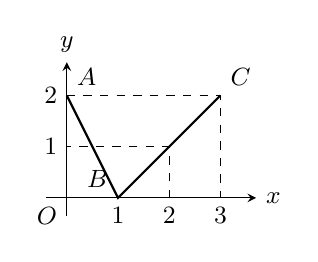
\begin{tikzpicture}[x=.65cm,y=.65cm,>=stealth,font=\small]
\draw[->](-.4,0)--(3.7,0)node[right]{$x$};\draw[->](0,-.35)--(0,2.65)node[above]{$y$};
\draw[thick](0,2)node[above right]{$A$}--(1,0)node[above left]{$B$}--(3,2)node[above right]{$C$};
\draw[dashed](0,2)--(3,2)--(3,0);\draw[dashed](2,0)--(2,1)--(0,1);
\node[below left]at(0,0){$O$};\foreach \x in {1,2,3}\node[below]at(\x,0){$\x$};
\foreach \y in {1,2}\node[left]at(0,\y){$\y$};\end{tikzpicture}\end{center}}
\renewcommand{\arraystretch}{1.2}

\newcommand{\PaperName}{B卷}
\begin{document}
\begin{center}{\Large\bfseries 高一数学期中教材改编练习卷（B）}\\[2mm]湘教版必修第一册\quad 120分钟\quad 满分150分\end{center}
班级\underline{\hspace{2.4cm}}\quad 姓名\underline{\hspace{2.4cm}}\quad 学号\underline{\hspace{2.4cm}}
\parttitle{一、单项选择题（共8小题，每题5分，共40分）}每题只有一个正确选项。
\par\noindent\begin{minipage}{\linewidth}
\q{1}{已知集合 $A=\{0,1,3\}$，$B=\{1,2,3,4\}$，则 $A\cup B=$（\quad）。}
\optsfour{$\{1,3\}$}{$\{0,2,4\}$}{$\{0,1,2,3,4\}$}{$\{0,1,2,4\}$}
\end{minipage}\par\smallskip
\par\noindent\begin{minipage}{\linewidth}
\q{2}{设 $x\in\R$，则“$x^2=9$”是“$x=3$”的（\quad）。}
\opts{充分而不必要条件}{必要而不充分条件}{充要条件}{既不充分又不必要条件}
\end{minipage}\par\smallskip
\par\noindent\begin{minipage}{\linewidth}
\q{3}{命题 $p$：$\forall x\in\R$，$x^2\ge x$。则 $p$ 的否定是（\quad）。}
\opts{$\exists x\in\R$，$x^2<x$}{$\forall x\in\R$，$x^2<x$}{$\exists x\in\R$，$x^2\le x$}{$\exists x\in\R$，$x^2>x$}
\end{minipage}\par\smallskip
\par\noindent\begin{minipage}{\linewidth}
\q{4}{已知 $a>0$，$b>0$，且 $ab=9$，则 $a^2+b^2$ 的最小值是（\quad）。}
\optsfour{$9$}{$6$}{$36$}{$18$}
\end{minipage}\par\smallskip
\par\noindent\begin{minipage}{\linewidth}
\q{5}{设 $A=\{-1,0,1\}$，$B=\{0,1,2\}$，下列对应中，能构成从 $A$ 到 $B$ 的函数的是（\quad）。}
\opts{$x\mapsto\dfrac1x$}{$x\mapsto\sqrt x$}{$x\mapsto x^2$}{$x\mapsto2x$}
\end{minipage}\par\smallskip
\par\noindent\begin{minipage}{\linewidth}
\q{6}{函数 $f(x)=\dfrac{\sqrt{x+1}}{x^2-4}$ 的定义域是（\quad）。}
\opts{$[-1,+\infty)$}{$[-1,2)\cup(2,+\infty)$}{$(-1,2)\cup(2,+\infty)$}{$(-\infty,-2)\cup(-2,2)\cup(2,+\infty)$}
\end{minipage}\par\smallskip
\par\noindent\begin{minipage}{\linewidth}
\q{7}{已知 $f(x)$ 是定义在 $\R$ 上的偶函数，当 $x\ge0$ 时，$f(x)=x^2-4x+1$，则 $f(-3)=$（\quad）。}
\optsfour{$-2$}{$22$}{$2$}{$-22$}
\end{minipage}\par\smallskip
\par\noindent\begin{minipage}{\linewidth}
\q{8}{若函数 $f(x)=-x^2+2ax$ 在区间 $[2,+\infty)$ 上单调递减，则 $a$ 的取值范围是（\quad）。}
\optsfour{$[2,+\infty)$}{$(-\infty,2)$}{$(2,+\infty)$}{$(-\infty,2]$}
\end{minipage}\par\smallskip

\newpage
\parttitle{二、多项选择题（共3小题，每题6分，共18分）}每题有多项正确。全部选对得6分，部分选对且无错项得3分，含错项或未选得0分。
\par\noindent\begin{minipage}{\linewidth}
\q{9}{已知 $a<b<0$，则下列结论正确的是（\quad）。}
\opts{$\dfrac1a>\dfrac1b$}{$a^2<b^2$}{$\dfrac ab>1$}{$-a<-b$}
\end{minipage}\par\smallskip
\par\noindent\begin{minipage}{\linewidth}
\q{10}{已知 $f(x)=x+\dfrac4x$，$x>0$，则下列结论正确的是（\quad）。}
\opts{对任意 $x>0$，$f(x)\ge4$}{$f(x)$ 在 $(0,2]$ 上单调递减}{$f(1)<f(4)$}{$f(x)$ 在 $x=4$ 时取得最小值}
\end{minipage}\par\smallskip
\par\noindent\begin{minipage}{\linewidth}
\q{11}{已知函数 $f:\R\to\R$ 满足 $f(x+y)=f(x)+f(y)$，且 $f(2)=6$，则（\quad）。}
\opts{$f(1)=6$}{$f(0)=0$}{$f(x)$ 是奇函数}{$f(6)=18$}
\end{minipage}\par\smallskip
\parttitle{三、填空题（共3小题，每题5分，共15分）}
\par\noindent\begin{minipage}{\linewidth}
\q{12}{若对任意 $x\in\R$，$-x^2+2x+k\le0$ 恒成立，则 $k$ 的取值范围为\blank。}
\end{minipage}\par\smallskip
\par\noindent\begin{minipage}{\linewidth}
\q{13}{已知 $f(x)=\begin{cases}x+2,&x\le0,\\x^2,&x>0,\end{cases}$ 则 $f(f(-1))=$\blank。}
\end{minipage}\par\smallskip
\par\noindent\begin{minipage}{\linewidth}
\q{14}{已知奇函数 $f(x)$ 的定义域为 $\R$，且在 $[0,+\infty)$ 上单调递增，则 $f(-2)$、$f(1)$、$f(3)$ 从小到大的排列为\blank。}
\end{minipage}\par\smallskip
\parttitle{四、解答题（共5小题，共77分）}解答须写出文字说明、证明过程或演算步骤。
\q{15}{（15分）设全集 $U=\R$，$A=\{x\mid-2\le x<5\}$，$B=\{x\mid x\ge t\}$，其中 $t\in\R$。\subq{1}{当 $t=1$ 时，求 $A\cap B$、$A\cup B$ 和 $\complement_U A$；}\subq{2}{若 $A\cap B=\varnothing$，求 $t$ 的取值范围。}}
\work{4.0cm}

\newpage
\q{16}{（15分）解下列关于 $x$ 的不等式，其中 $m\in\R$。\subq{1}{$-x^2+3x+4>0$；}\subq{2}{$x^2-(m+2)x+2m\ge0$。}}
\work{6.7cm}
\q{17}{（17分）已知 $f(x)$ 是定义在 $\R$ 上的奇函数，当 $x\ge0$ 时，$f(x)=x^2+2x$。\subq{1}{求 $f(0)$ 和 $f(-2)$；}\subq{2}{求 $f(x)$ 在 $(-\infty,0)$ 上的解析式；}\subq{3}{用函数单调性的定义证明 $f(x)$ 在 $\R$ 上单调递增。}}
\work{7.0cm}

\newpage
\q{18}{（17分）完成下列问题。\subq{1}{计算 $16^{\frac34}+8^{-\frac23}$；}\subq{2}{已知幂函数 $f(x)=x^\alpha$ 的图象经过点 $(8,2)$，求其解析式及定义域；}\subq{3}{判断（2）中函数的奇偶性，写出其单调区间，并用定义证明它在 $(0,+\infty)$ 上的单调性。}}
\work{6.6cm}
\q{19}{（13分）已知函数 $f(x)=a^{|2x+1|}$，其中 $a>0$ 且 $a\ne1$，并且 $f(0)=2$。\subq{1}{求 $a$ 的值；}\subq{2}{写出 $f(x)$ 的单调区间及相应的增减性，并求值域；}\subq{3}{解不等式 $f(x)\le8$。}}
\work{6.5cm}
\end{document}
